\section{\textsc{Экспериментальные результаты}}

В качестве примера сначала рассмотрим геомагнитную бурю 25-26 августа 2018 года с индексом G3, которая является одним из самых сильных гелиогеофизических явлений за период 24-го цикла солнечной активности.
Причиной этой бури является корональный выброс массы Солнца, произошедший 20 августа 2018 года и достигнувший Земли в течение 5 дней.
На рис. \ref{fig-dst1808} изображена динамика индекса DST за август 2018 года, которая была получена при помощи всемирной базы данных геомагнитизма \cite{WDC}. 
Значение индекса достигает своего минимума (примерно -180 нТл) 26 августа в 07:15 UT, после чего начинается фаза восстановления бури.   
\begin{figure}[h]
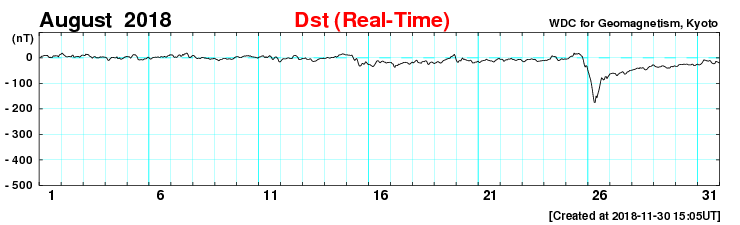
\includegraphics[width=\textwidth]{fig/dst1808.png}    
\caption{Динамика индекса DST за август 2018 года.}
\label{fig-dst1808}      
\end{figure} 

На рис. \ref{fig-2018-237-238-07-45} (c) и (d) изображены глобальные распределения полной ошибки позиционирования в 07:45 UT для 25 (перед бурей) и 26 (главная фаза бури) августа 2018 года, соответственно. 
Панелям (a) и (c) соответствуют глобальные распределения вариаций TEC, отфильтрованных в диапазоне периодов 10-20 мин.   
Эти вариации были получены при помощи сервиса автоматического сбора и обработки данных ГНСС SIMuRG \cite{Yasyukevich2020}.  
\begin{figure}[h]
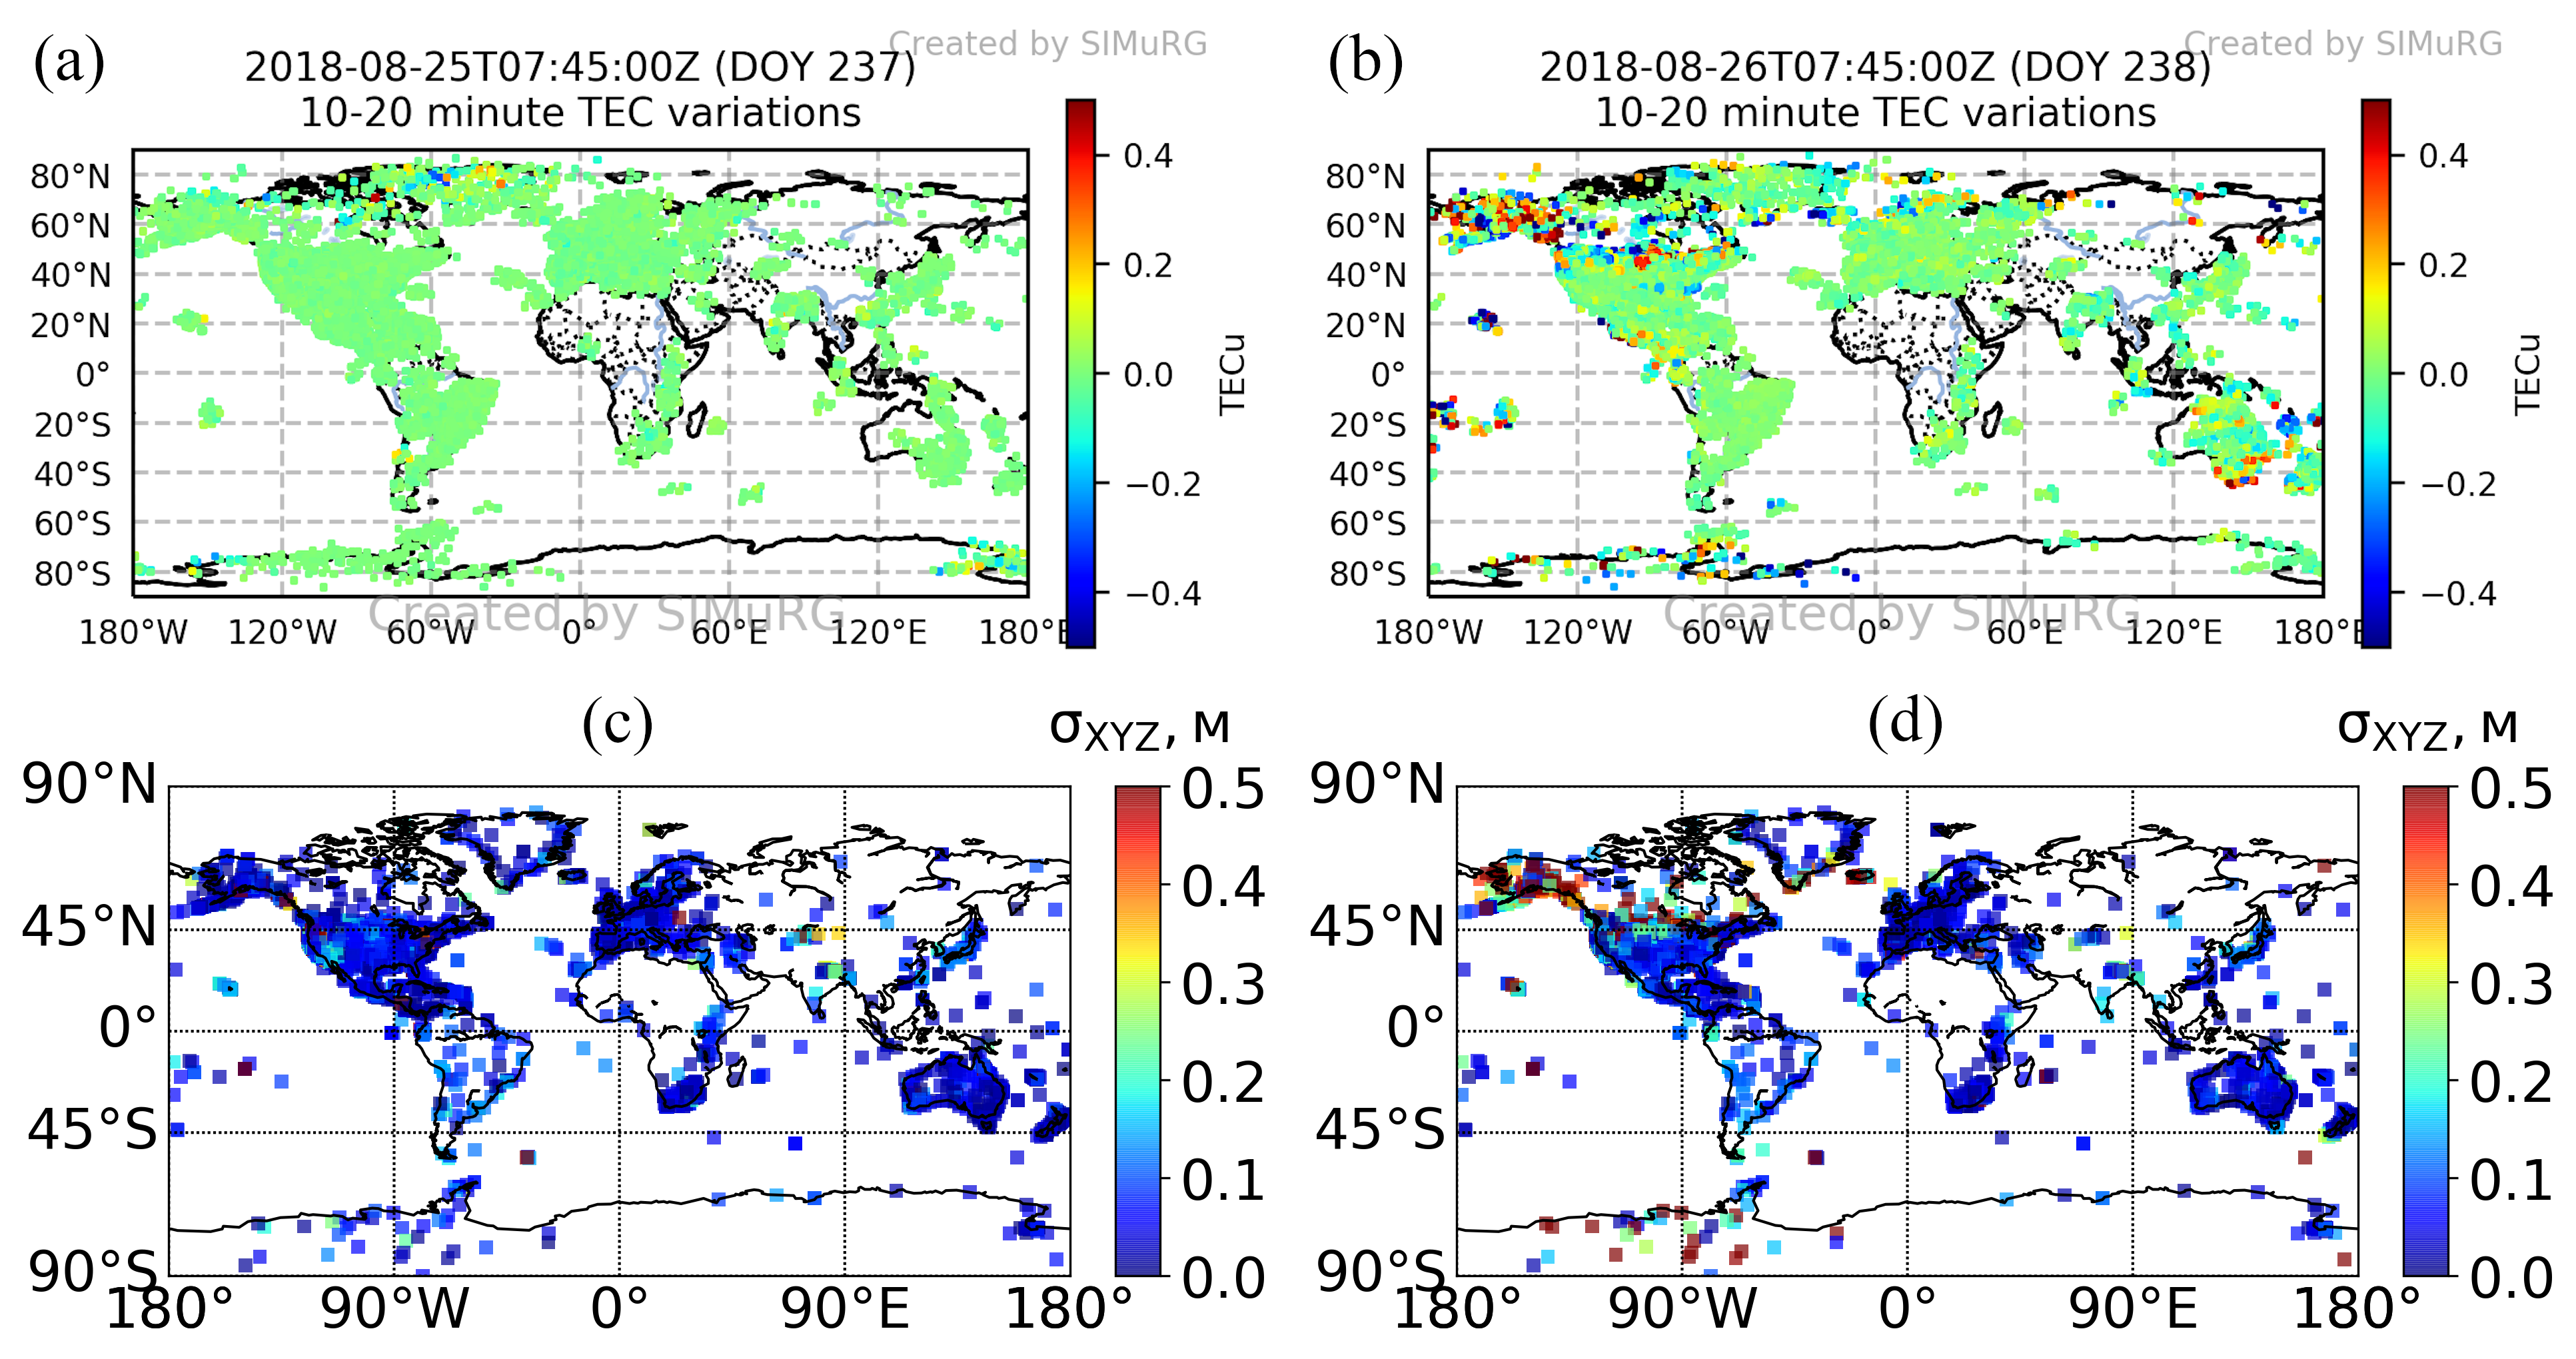
\includegraphics[width=\textwidth]{fig/2018-237-238-07-45.png}    
\caption{Глобальные распределения вариаций TEC (a-b) и полной ошибки позиционирования (c-d) в 07:45 UT для 25 (a-c) и 26 (b-d) августа 2018 года.}
\label{fig-2018-237-238-07-45}      
\end{figure} 

На рис. \ref{fig-2018-237-238-07-45} (b) во время главной фазы бури заметно значительное увеличение значений вариаций TEC в областях, вытянутых вдоль аврорального овала, как в северном, так и в южном полушариях.
В североамериканском секторе сильные возмущения достигают вплоть до 40\degree N.
Повышенные значения вариаций TEC также наблюдаются в экваториальной области.
В этих же регионах на рис. \ref{fig-2018-237-238-07-45} (d) заметно увеличение значений полной ошибки позиционирования, которые не были зарегистрированы в период до бури.
Для некоторых приёмных станций величина ошибки превосходит 0,5 м, по сравнению с 0,1 м в спокойный день. 

На рис. \ref{fig-2018-237-238} изображены зависимости усреднённой полной ошибки позиционирования от времени и широты для восточного (a-c) и западного (b-d) полушарий.
Панелям (a) и (b) соответствует 25 августа, а (c) и (d) -- 26 августа.
Горизонтальные синие полосы (нулевые значения) указывают на отсутствие данных.
Во-первых, следует обратить внимание, что решение PPP, полученное при помощи GAMP, имеет период схождения примерно от 0 до 2 UT.
Поэтому это время можно не рассматривать.
Согласно результатам на рис. \ref{fig-2018-237-238} (a) и (b), в спокойный день характерные значения ошибки в большинстве регионов не превышают 0,1 м.
Однако в западном полушарии на широтах 30-60\degree N значения ошибки больше и достигают примерно 0,3 м.
Это увеличение, скорее всего, связано с особенностью обработки данных, например, из-за геометрии используемых спутников. 
\begin{figure}[h]
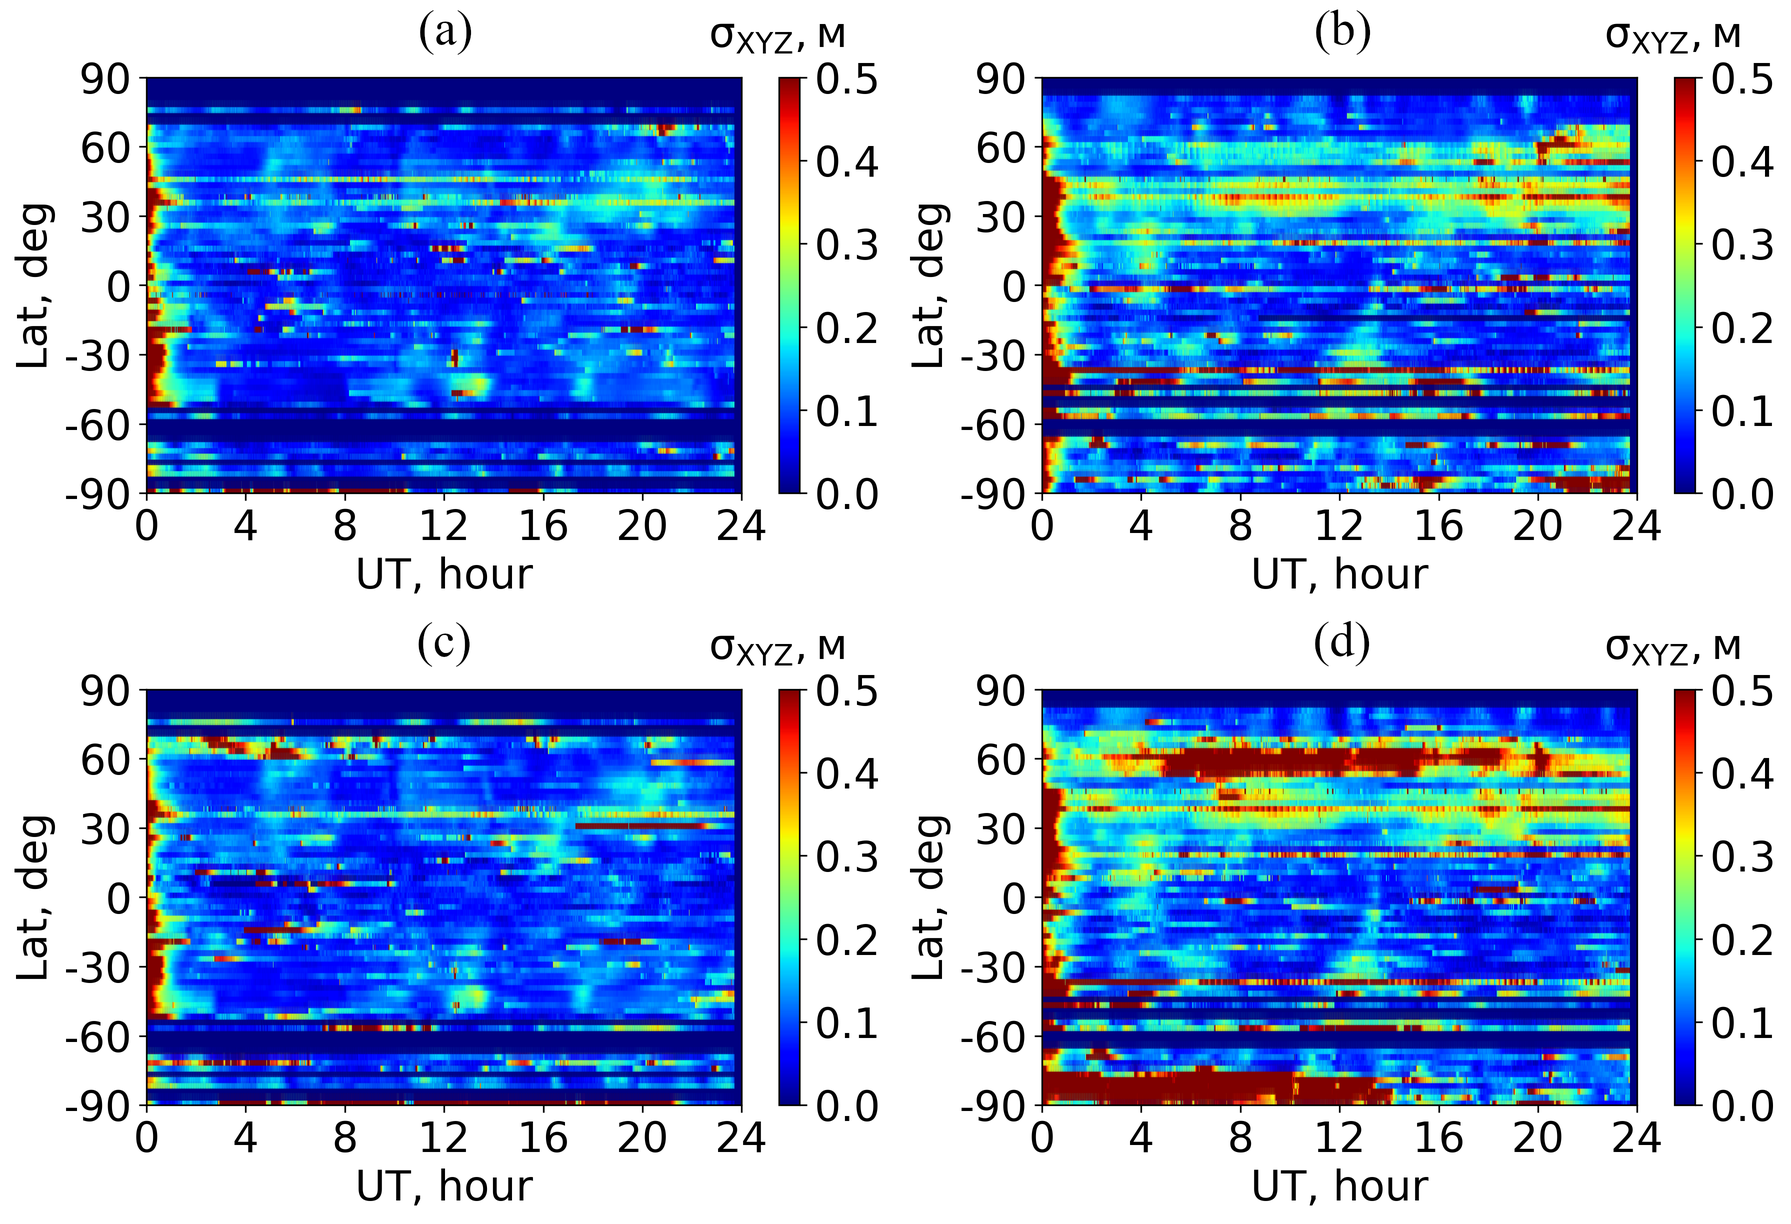
\includegraphics[width=\textwidth]{fig/2018-237-238.png}    
\caption{Зависимости усреднённой полной ошибки позиционирования от времени и широты 25 (a-b) и 26 (c-d) августа 2018 года для восточного (a-c) и западного (b-d) полушарий.} 
\label{fig-2018-237-238}      
\end{figure} 

25 августа после 20:00 UT можно заметить небольшое увеличение средней ошибки на широтах 65-75\degree N как в восточном, так и в западном полушариях. 
В течение всего дня 26 августа в североамериканском секторе отчётливо наблюдается резкое снижение точности PPP.
Значения средней ошибки значительно превышают 0,5 м.
Помимо этого, заметный рост ошибки виден на высоких широтах в южном полушарии до примерно 14 UT.
В восточном полушарии ухудшение точности позиционирования наблюдается до полудня на широтах 60-70\degree N.

Следующим рассмотренным гелиогеофизическим событием является магнитная буря 21-23 июня 2015 года с индексом G4.
Согласно каталогу \cite{SOHO}, источниками этой бури являются несколько корональных выбросов массы из активной области Солнца 12371.
На рис. \ref{fig-dst1506} изображена динамика индекса DST за июнь 2015 года.
Значения индекса достигают своего минимума (примерно -200 нТл) в начале 23 июня.
Однако ионосферные возмущения 22 июня в основном связаны с выбросом типа Halo (1350 км/c), произошедшим в результате вспышки M2.7 с максимумом в 02:34 UT, который стал причиной внезапных магнитных бурь примерно в 05:45 UT и 18:30 UT.
\begin{figure}[h]
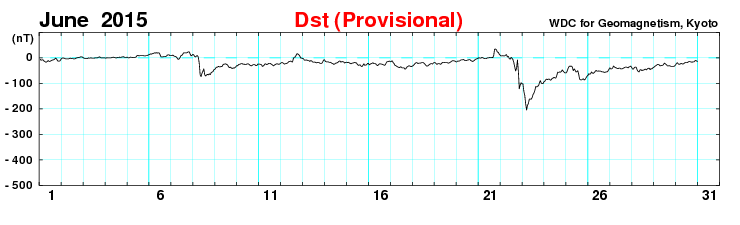
\includegraphics[width=\textwidth]{fig/dst1506.png}    
\caption{Динамика индекса DST за июнь 2015 года.}
\label{fig-dst1506}      
\end{figure} 

На рис. \ref{fig-2015-172-173-19-00} изображены глобальные распределения полной ошибки позиционирования (c-d), а также вариаций TEC (a-b) в 19:00 UT для 21 (a-c) и 22 (b-d) июня 2015 года. 
Аналогично предыдущему случаю здесь значительное увеличение значений вариаций TEC наблюдается в областях, вытянутых вдоль аврорального овала, как в северном, так и в южном полушариях. 
Однако можно заметить, что ``интенсивность'' и долготная протяжённость этих областей гораздо больше, чем для бури 25-26 августа 2018 года.
Абсолютные значения вариаций TEC достигают более 0,4 TECU вплоть до азиатского региона. 
Эти области также хорошо пространственно коррелируют с областями увеличения полной ошибки позиционирования на рис. \ref{fig-2015-172-173-19-00} (d). 
Стоит отметить, что SIMuRG использует большее количество серверов с данными региональных сетей ГНСС (всего задействовано порядка 6000 приёмных станций \cite{Yasyukevich2020}).
По этой причине эффект в наиболее интересной зоне (североамериканском секторе) на рис. \ref{fig-2015-172-173-19-00} (c) и (d), к сожалению, ограничен лишь её контуром.  

На рис. \ref{fig-2015-172-173} изображены зависимости усреднённой полной ошибки позиционирования от времени и широты для восточного (a-c) и западного полушарий. 
Панелям (a) и (b) соответствует 21 июня, а (c) и (d) -- 22 июня.
Вертикальной пунктирной линией отмечено время начала внезапной магнитной бури в 18:30 UT. 
В этом случае характерные значения средней ошибки аналогично составляют менее 0,5 м (даже менее 0,1-0,3 м).
22 июня на рис. \ref{fig-2015-172-173} (c) и (d) отчётливо видно резкое ухудшение точности позиционирования после 18:30 UT в северном полушарии на широтах 65-75\degree N, а также в южном полушарии на широтах 75-90\degree S.
Здесь величина ошибки увеличивается в несколько раз и превышает 0,5 м.
Помимо этого, можно заметить экваториальное ``распространение'' ошибки со временем.
В западном полушарии на рис. \ref{fig-2015-172-173} (d) такое ``распространение'' наблюдается примерно до 50\degree N.
На этой широте максимум ошибки находится примерно в 20 UT.
В восточном же полушарии на рис. \ref{fig-2015-172-173} (c) наблюдается похожая картина с увеличением ошибки позиционирования после 18:30 UT, но не так ярко из-за меньшего количества станций.
\begin{figure}[h]
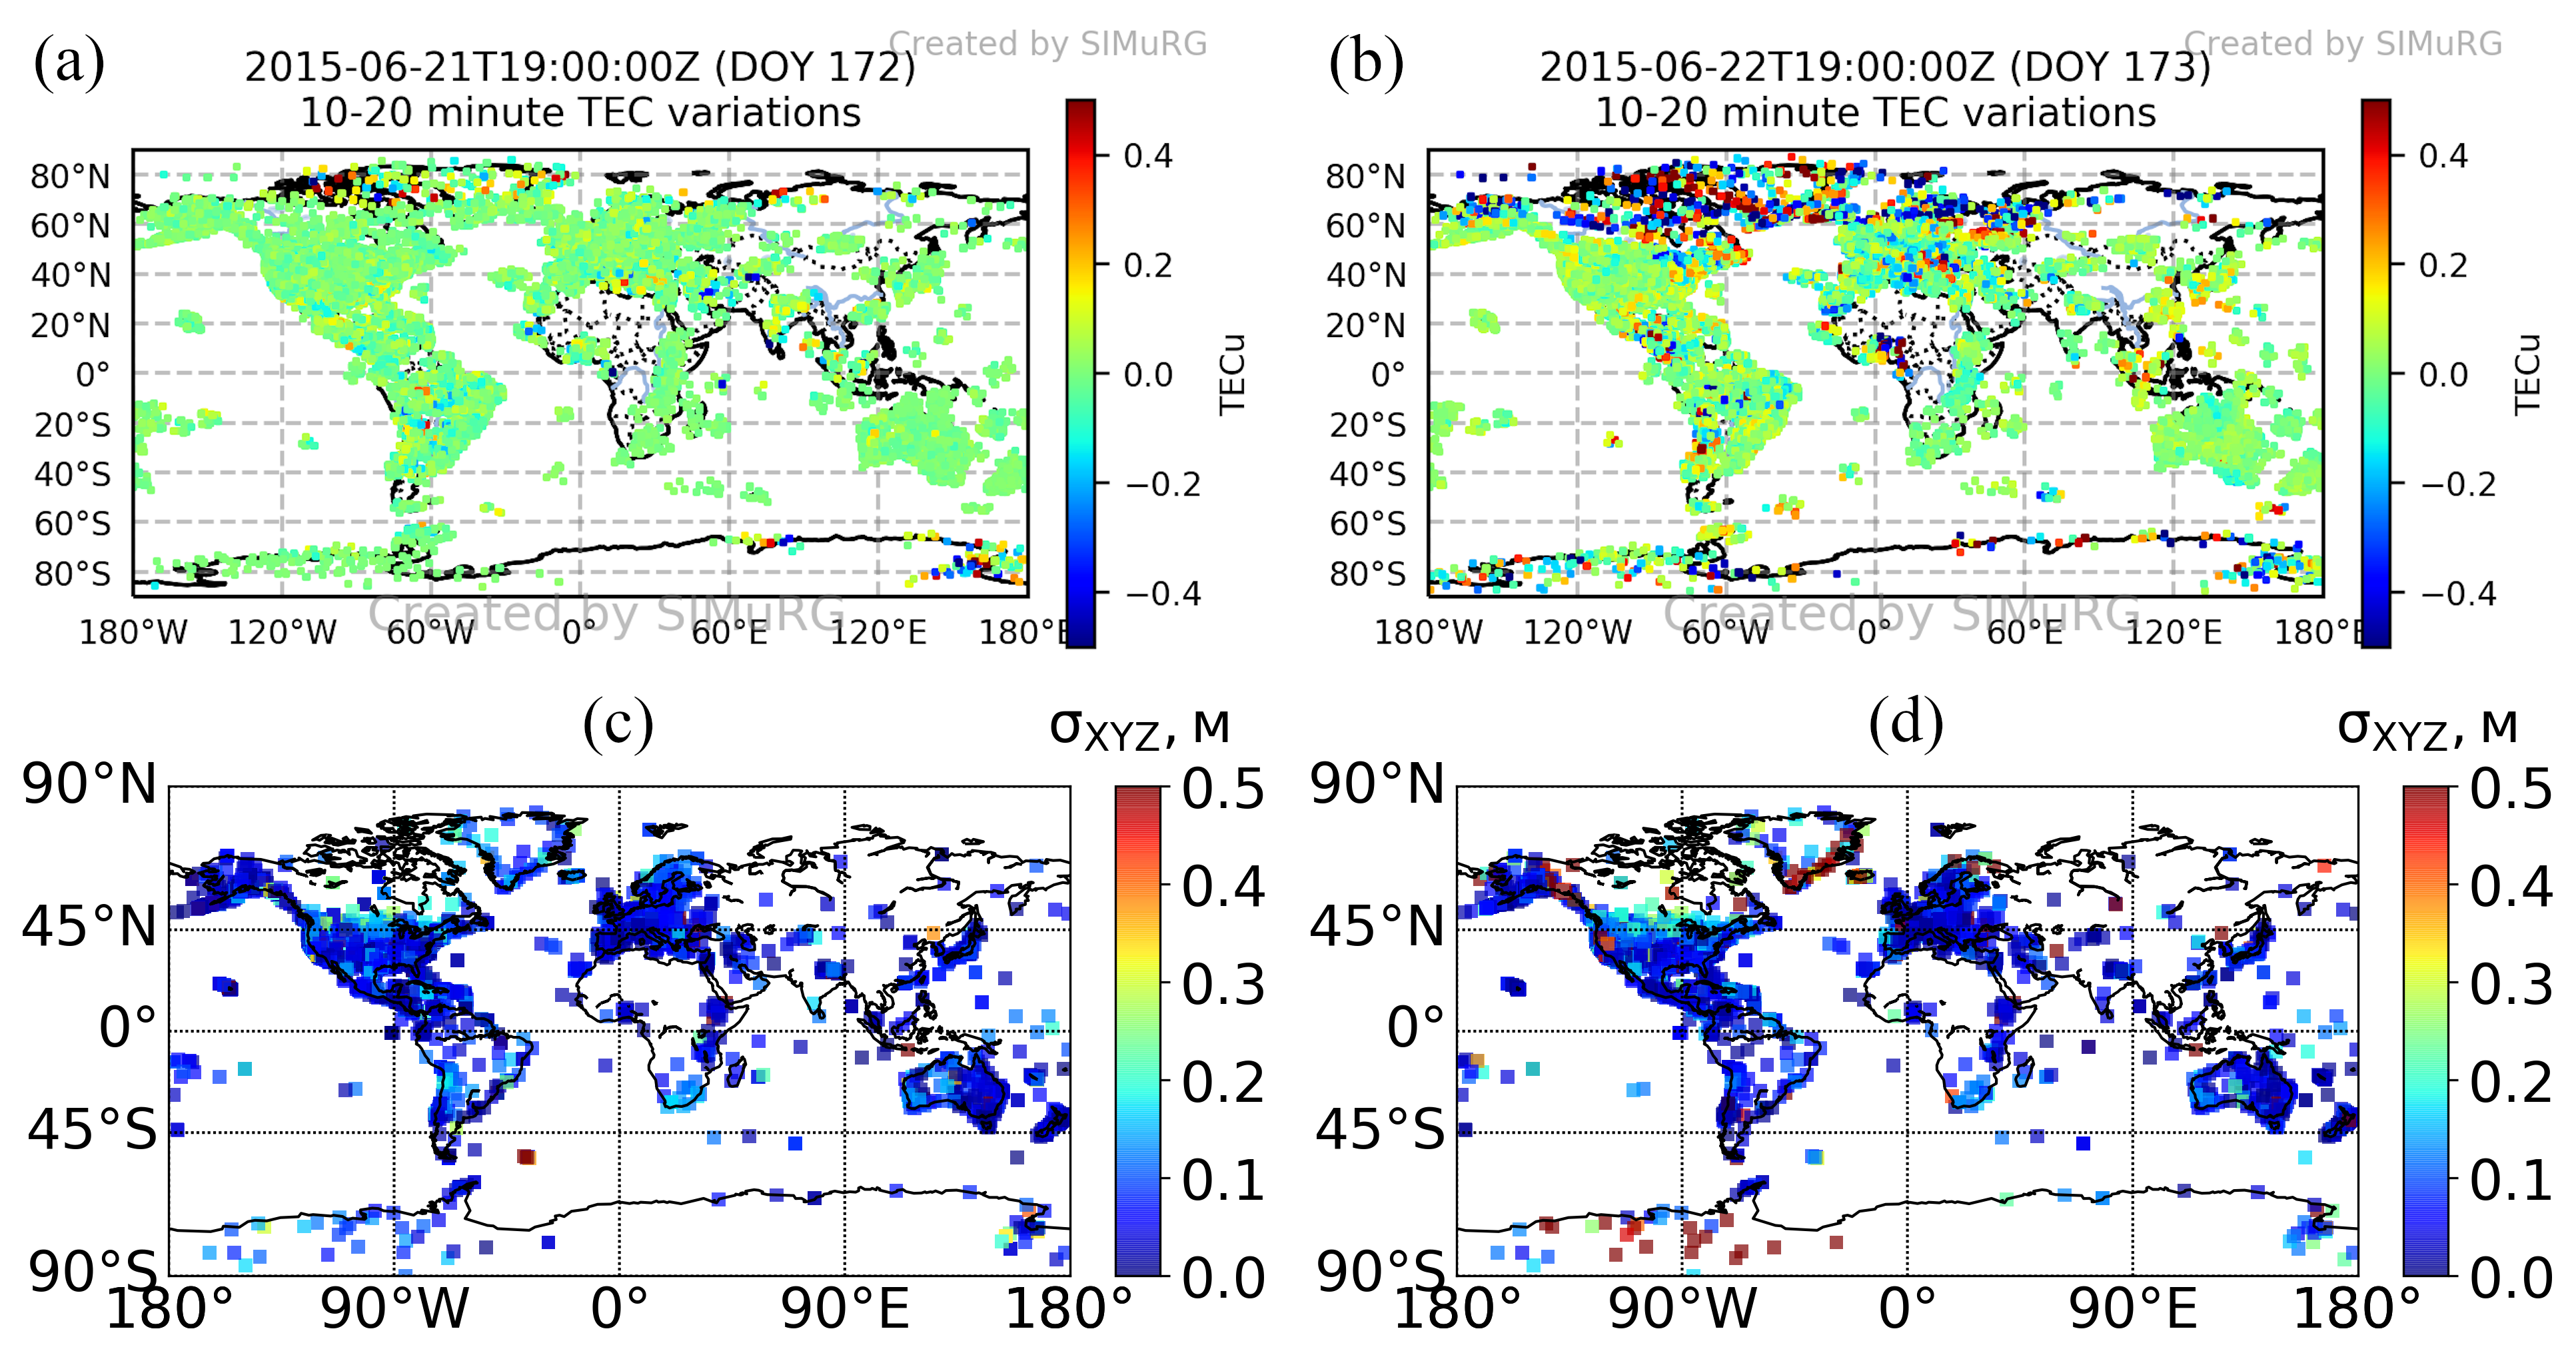
\includegraphics[width=\textwidth]{fig/2015-172-173-19-00.png}    
\caption{Глобальные распределения вариаций TEC (a-b) и полной ошибки позиционирования (c-d) в 19:00 UT для 21 (a-c) и 22 (b-d) июня 2015 года.}
\label{fig-2015-172-173-19-00}
\end{figure}
\begin{figure}[h]
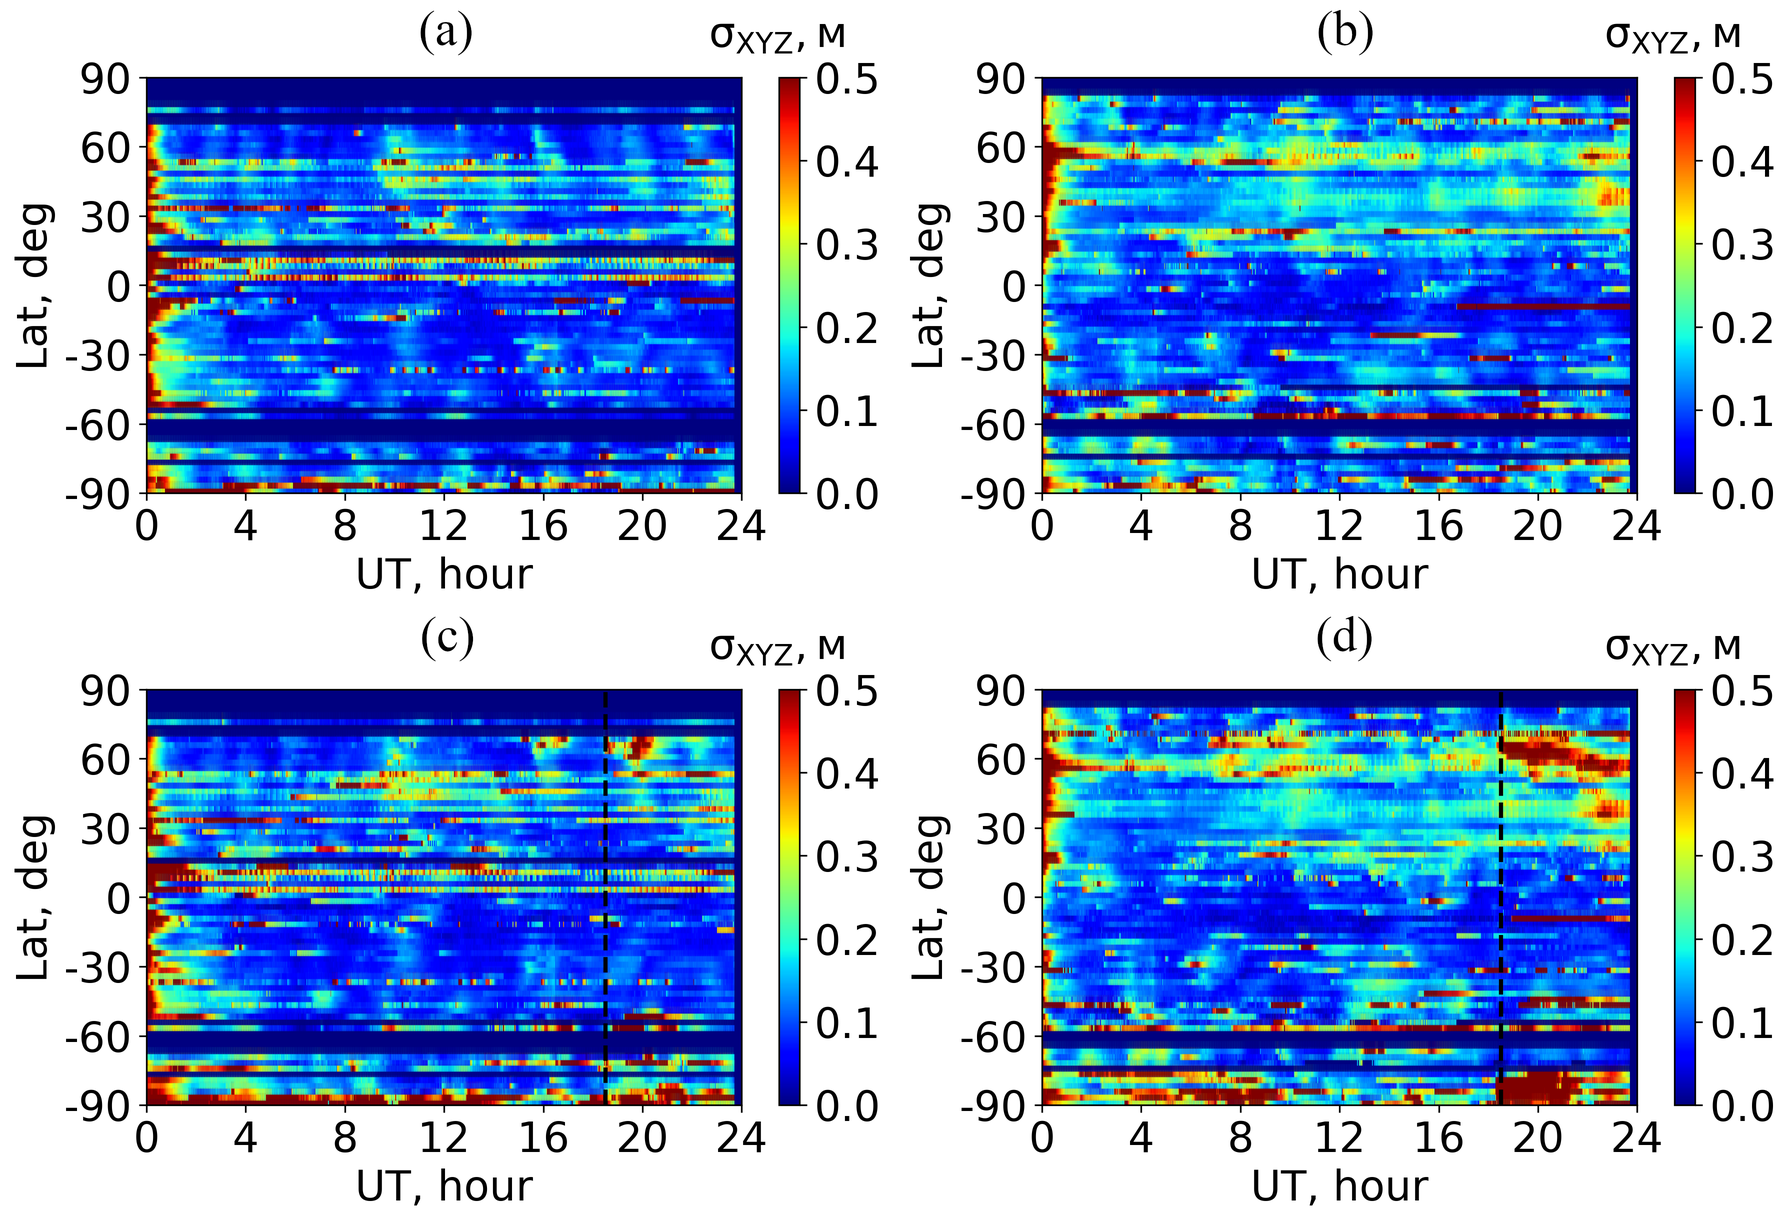
\includegraphics[width=\textwidth]{fig/2015-172-173.png}    
\caption{Зависимости усреднённой полной ошибки позиционирования от времени и широты 21 (a-b) и 22 (c-d) июня 2015 года для восточного (a-c) и западного (b-d) полушарий. Вертикальная пунктирная линия соответствует 18:30 UT.} 
\label{fig-2015-172-173}      
\end{figure} 